\documentclass[border=6pt]{standalone}
\usepackage{pgfplots}
\pgfplotsset{compat=1.17}
\usepackage{mathptmx}
\definecolor{navy}{RGB}{20,52,110}
\definecolor{accent}{RGB}{14,110,120}
\definecolor{orange}{RGB}{200,110,30}
\definecolor{gray70}{RGB}{130,130,130}
\begin{document}
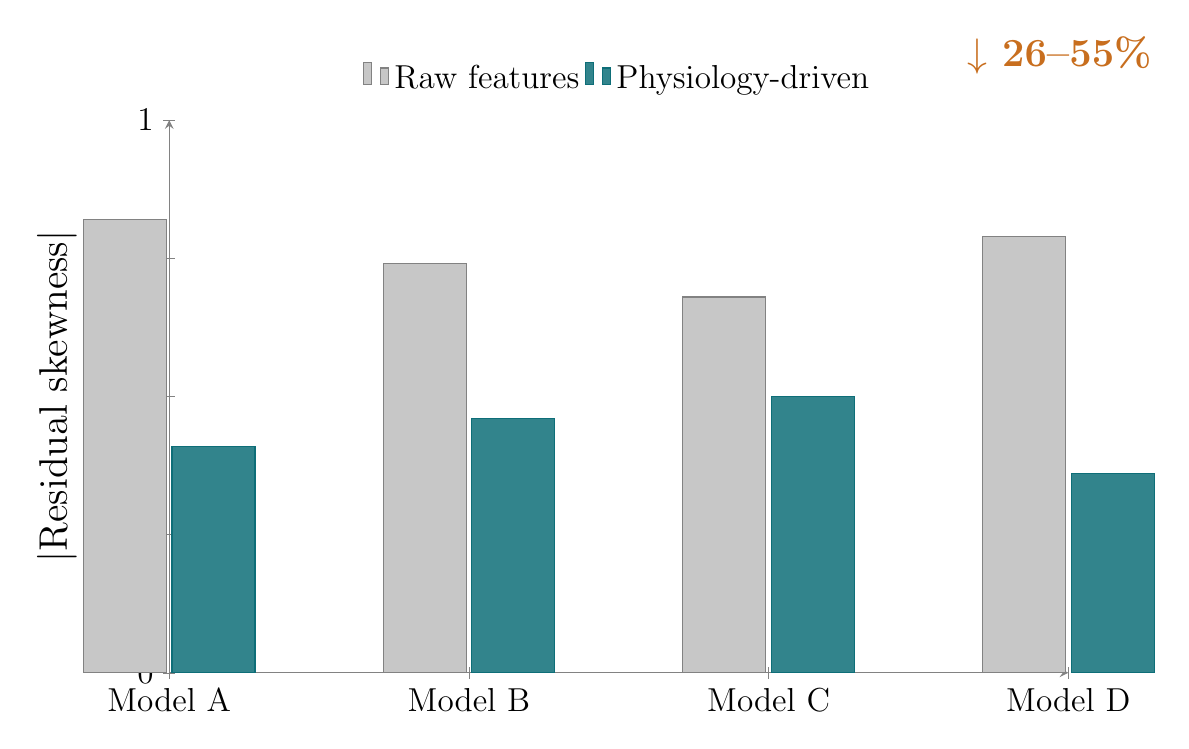
\begin{tikzpicture}
\begin{axis}[
    width=13cm, height=8.6cm,
    ybar,
    bar width=30pt,
    ymin=0, ymax=1.0,
    ytick={0,0.25,0.5,0.75,1.0},
    ylabel={\Large $|$Residual skewness$|$},
    ylabel style={font=\large},
    symbolic x coords={M1,M2,M3,M4},
    xtick=data,
    xticklabels={Model A, Model B, Model C, Model D},
    xticklabel style={font=\large},
    yticklabel style={font=\large},
    axis lines=left,
    axis line style={gray70},
    tick style={gray70},
    legend style={font=\large, at={(0.5,1.12)}, anchor=north, legend columns=2, draw=none},
    clip=false,
]
\addplot[draw=gray70, fill=gray70!45] coordinates {(M1,0.82)(M2,0.74)(M3,0.68)(M4,0.79)};
\addplot[draw=accent, fill=accent!85] coordinates {(M1,0.41)(M2,0.46)(M3,0.50)(M4,0.36)};
\legend{Raw features, Physiology-driven}
\end{axis}
\node[font=\Large\bfseries, color=orange, anchor=north east] at (12.6,8.2) {$\downarrow$ 26--55\%};
\end{tikzpicture}
\end{document}
